\documentclass[letterpaper,10pt]{article}
\usepackage[margin=1in]{geometry}
\usepackage{mathpazo}
\usepackage{color}
\usepackage[small,compact]{titlesec}
\usepackage{caption}
\usepackage{hyperref}
\usepackage{graphicx}
\usepackage{multicol}
\usepackage{dblfnote}

\newcommand{\mycaption}[1]{\caption{\small{#1}}}

\newcommand{\squishlist}{\begin{list}{$\bullet$}
  {\setlength{\itemsep}{0pt}
    \setlength{\parsep}{3pt}
    \setlength{\topsep}{3pt}
    \setlength{\partopsep}{0pt}
    \setlength{\leftmargin}{1.5em}
    \setlength{\labelwidth}{1em}
    \setlength{\labelsep}{0.5em}}}

\newcommand{\squishend}{\end{list}}

\makeatletter
\newenvironment{tablehere}
{\def\@captype{table}}
{}
\newenvironment{figurehere}
{\def\@captype{figure}}
{}
\makeatother

\title{libtorque: Portable Multithreaded Continuations\\
for Scalable Event-Driven Programs}
\author{Nick Black and Richard Vuduc \\
Georgia Institute of Technology \\
nickblack@linux.com, richie@cc.gatech.edu
}
\date{}

\newcommand{\TODO}[1]{{\color{red}\textbf{#1}}}

%%%%%%%%%%%%%%%%%%%%%%%%%%%%%%%%%%%%%%%%%%%%%%%%%%%%%%%%%%%%%%%%%%%%%%%%
\begin{document}
%%%%%%%%%%%%%%%%%%%%%%%%%%%%%%%%%%%%%%%%%%%%%%%%%%%%%%%%%%%%%%%%%%%%%%%%
\maketitle
\begin{abstract}
Since before even 4.4BSD or POSIX.1\footnote{\texttt{select(2)} first showed up in 4.2BSD, \texttt{poll(2)} in
SVR4.}, programming via events and continuations has marked best UNIX practice
for handling multiplexed I/O\footnote{As canonicalized within the books of W. Richard Stevens~\cite{Stevens03}.}.
The idiom's programmability was proved sapient astride a decade's architectures
and operating systems, as \textit{libevent}~\cite{Mathewson09}, \textit{libev},
Java NIO and others achieved ubiquity among network applications. Academic~\cite{Welsh02} and proprietary systems
have responded to multiprocessor economics with threaded callback engines, but
such I/O cores remain rare in open source: Firefox uses
multiple functionally-decomposed event loops, \texttt{nginx} multiple processes
with static load distribution, and Apache's \texttt{mpm-worker} variant a thread
per connection. Economic employment of even COTS (Consumer Off-The-Shelf) hardware already
requires concurrent workloads, and manycore's march into the data
center still more: dynamic parallelism as rule rather than exception. The community agrees that UNIX network programming
must change~\cite{Drepper06}~\cite{Jacobson06}, but consensus of direction remains
elusive~\cite{Kegel2010}~\cite{Varghese05}. We present our open source,
portable \textit{libtorque} library, justify the principles from which it was derived, extend previous threaded cores through aggressively
exploiting details of memories, processors, and their interconnections (as detected at runtime), and imply a
new state-of-the-art in architecturally-adaptive, high-performance systems
programming. Built with scalability (in both the large and small), low latency,
and faithfulness to UNIX idiom as guiding lights, \textit{libtorque} subsumes the functionality of existing I/O frameworks (for which we provide compatibility
wrappers) despite superior performance across most loads and apparatus.
\end{abstract}
\begin{multicols}{2}
%=======================================================================
\section{Intro}
\label{sec:intro}
%=======================================================================
It's a rare and rather lucky program which spends most of its wall time
calculating. Whether an interactive application, a desktop widget, or a network
server, relative eternities are made up of waiting for, shuffling, and
signaling the presence of data. Spinning on event readiness implies ineffective
use of processor and power, motivating event registration and data readiness
notification schemes (of which blocking I/O---with or without a timeout---can be
thought the \textit{uniplex} special case. Each thread has a single channel,
bound to a single source). This concept forms the essential \textit{omphalos} of
POSIX's system interfaces: Pthread condition variables, asynchronous I/O, and
humble \texttt{read(2)} can all be interpreted as some mapping between threads
and event sources, with the goal always of sleeping as much as local service
requirements allow. Every non-trivial program will use them at least once.

Given our definition of blocking I/O, spinless employ of multiple event sources
requires either multiple threads or multiplexed, non-blocking (possibly
asynchronous, i.e.\ kernel-demultiplexed) I/O. The former solution, at the cost
of $O(n)$ threads and $O(n)$ context switches for $n$ event sources, retains
the simplicity and streamline (thanks to the absence of any multiplexing
interfaces) of blocking. With the advent of Linux's NPTL and FreeBSD's libthr,
this method has seen a resurgence, and even argument \textit{a posteriori}
that its performance might exceed that of multiplexed I/O~\cite{vonBehren03}.
That this is possible---that $O(n)$ time and space costs are negated by
multiplexing overhead, as evidenced in~\cite{Tyma08}---shows how much room for
improving non-blocking I/O solutions exists on modern machines. We enumerate and address five possible overheads:
memory effects, multiplex setup (``enplexing''?), synchronization within the system call,
walking of the event table, and copying the results to userspace. We illustrate
several ways I/O-intensive applications can (and \textit{libtorque} does) make
effective use of system architecture properties. We show that a tradeoff exists
between dynamic balance under arbitrary load and synchronization costs, and
how it might be optimized. The result is as powerful, flexible, and scalable as
POSIX.1b Asynchronous I/O~\cite{Posix1b}, Windows's I/O Completion Ports~\cite{Russinovich09}
or Solaris's Event Completion Framework~\cite{Solaris06}, but makes better use
of modern, complex architectures (see~\cite{Veal07} and~\cite{Guo08} for the
profound effects of multicore and CMT on network servers). We see it as a viable successor to or merge
candidate for \textit{libev}, especially given its compatibility interface\footnote{A
tradition begun with \textit{libev}'s similar wrapper for \textit{libevent}.}.

%=======================================================================
\section{Architecture and APIs}
%=======================================================================
\textit{libtorque} assumes exclusive use of all $n$ processors in its cpuset (as inherited from the creating thread, which
ought prune processors prior to calling \texttt{libtorque\_init()} if appropriate).
$n$ threads are created via exponential bloom (requiring $O(n)$ work in $O(\log{n})$ depth),
and use hard affinity to preclude expensive migrations (see~\cite{Porterfield08}
and Section~\ref{sec:queuedist} for justification). Each thread probes its
processor and attached memories, collaboratively establishing a map of hardware.
Stacks and event queues---optimal in number and placement---are created,
and entered via the method of \texttt{sigaltstack(2)} trampoline~\cite{Engelschall00}. Threads begin the event loop,
the signal mask is reset, and control is returned to the caller.

%\textit{libtorque} implements an event-differentiated kernel. All
%threads loop within the same lowest level function; functional and data
%decomposition is strictly temporary and dynamic (though, as we will see, effort
%is made to maintain locality). One thread runs per available processor
%(\textit{libtorque} makes full use of container and cpuset functionality), using hard affinity
%to avoid migration costs~\cite{Porterfield08}. Preferably, the application has
%been exclusively allocated some cpuset. If some other process is scheduled onto
%one of our CPUs, the corresponding thread will simply run less. This is, to a limit,
%desirable: were it scheduled onto some other processor sharing its event queue,
%those two would simply contend 
% Sufficient
%sharing of event sources means there will be progress, if possible, without some given
%thread). Cpusets are inherited from parent threads, so \textit{libtorque} can be
%restricted by pruning the active set prior to \texttt{libtorque\_init()}.
\setlength{\abovecaptionskip}{0pt}
\setlength{\belowcaptionskip}{0pt}
\begin{figurehere}
\centering
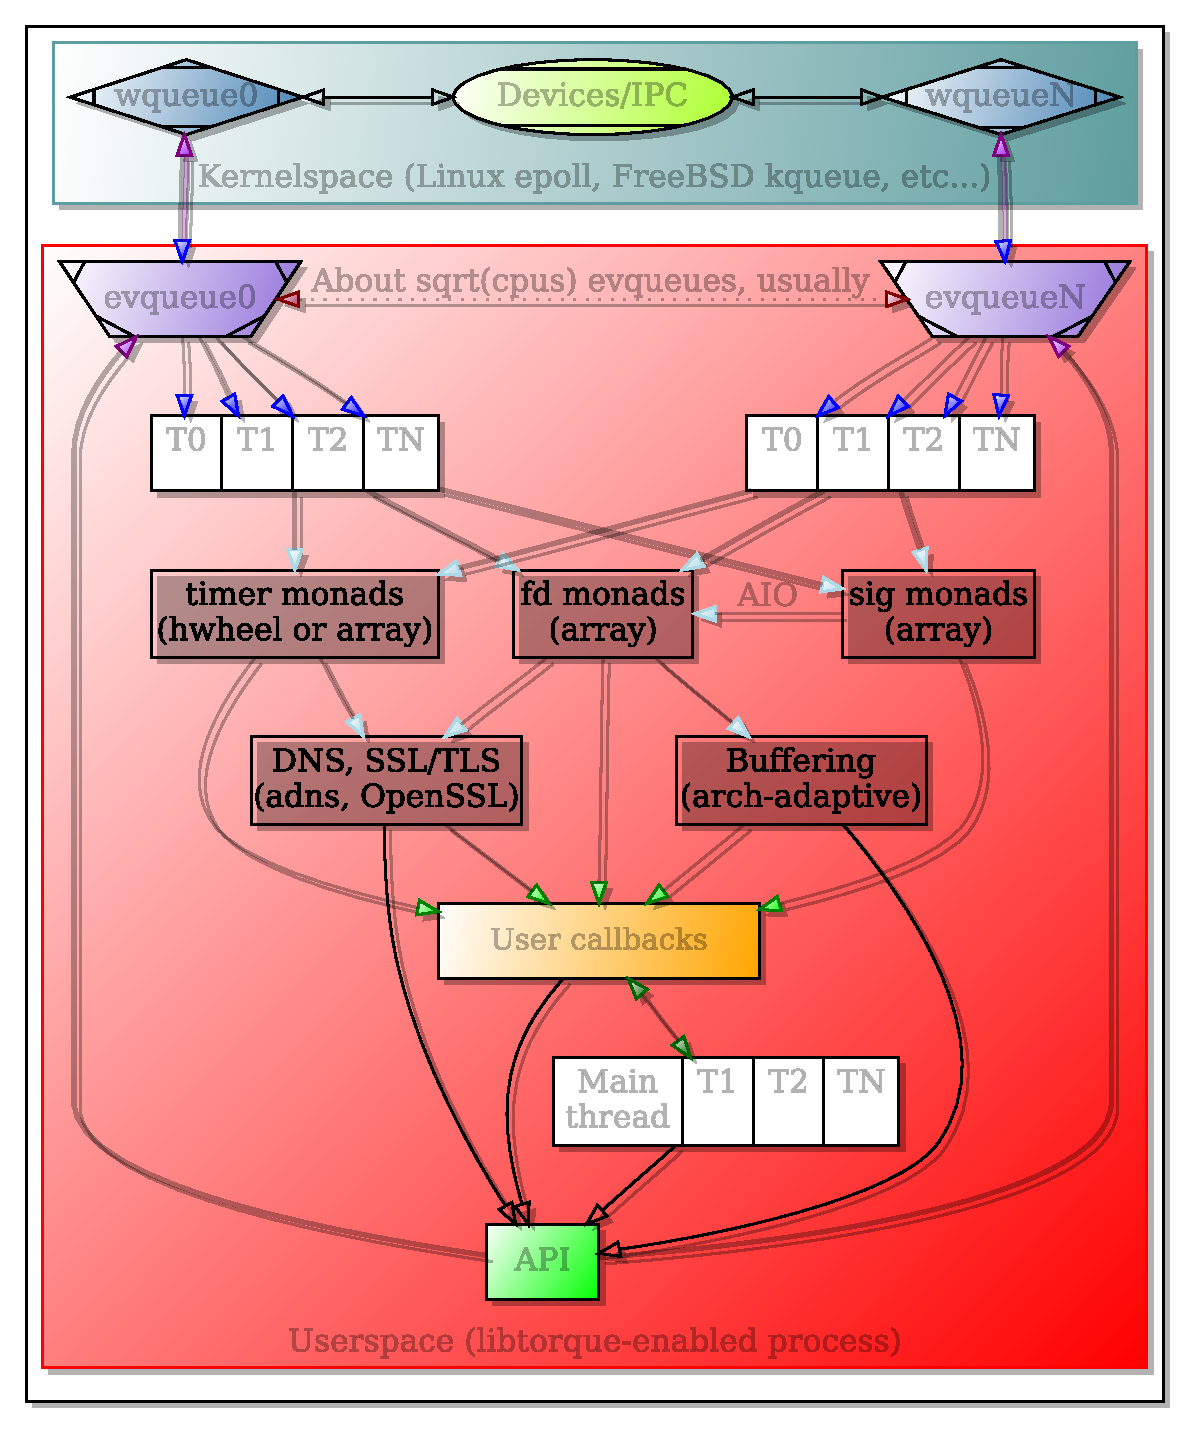
\includegraphics[width=\columnwidth]{doc/paper/libtorque}
\mycaption{Architecture of a \textit{libtorque}-enabled process.}
\label{fig:processArch}
\end{figurehere}
All entry points are thread-safe\footnote{None are async(signal)-safe.}. All save the constructor (\texttt{libtorque\_init()})
and destructors (\texttt{libtorque\_stop()} and \texttt{libtorque\_block()})
operate in $O(1)$ time and space. All are lock-free throughout userspace (the kernel
itself locks in some cases) and usually wait-free\footnote{\textit{Lock-free} implies system progression, while
\textit{wait-free} requires progression from each thread.}. This arises
from the kernel's synchronization of new file descriptors (ensuring no
two entities are given the same descriptor), the kernel's synchronization of
event notification state with descriptor closings (closing a descriptor
atomically removes it from all queues), and the kernel's synchronization of
event queue modifications and retrievals.
\subsection{Currying as de-layering}
Network programming abounds with task idioms. \textit{libtorque} implements
several ((de)compression, X.509-based authentication and symmetric encryption via
OpenSSL~\cite{OpenSSL}, and asynchronous hostname resolution via GNU adns~\cite{Adns})
in a fully layerable fashion reminiscent of SVR4 STREAMS~\cite{Ritchie84}. This
is easily achieved via the generic marshaling technique known as \textit{currying}.
In addition, several types of buffering are provided. \textit{libtorque}'s extensive
system detection allows (possibly NUMA and/or heterogeneous) memories' (usually
multiple) page sizes to be taken into consideration for buffer sizing and
even placement. Since buffers are highly unlikely to be truly shared among
threads or to exhibit temporal locality throughout the threads's life, we
\textit{color} both threads' stacks and buffers, of which each thread keeps a
properly-formed pool. This aggressive mobilization of the memory hierarchy is
a major reason why \textit{libtorque} makes use of hard affinity.
\subsection{Callback semantics}
In the interests of simplicity, robustness and ease of porting existing code,
callbacks are restricted as little as possible. They may spawn child programs
or helper threads, close arbitrary file descriptors, and call back into a
\textit{libtorque} instance. Fatal signals continue to terminate the process,
unless caught elsewhere. Some requirements are unavoidable:
\squishlist
\item Blocking calls must be avoided. Numerous systems exist to automatically
dispatch blocking I/O~\cite{Crameri06}, and \textit{libtorque} provides
the facilities to support them. Any code written with performance in
mind is almost certainly already using non-blocking or asynchronous I/O.
\item Callbacks must not freely operate on event sources registered with libtorque,
save to \texttt{close(2)} file descriptors; this is safe due to the atomicity properties described above.
\item Obviously, the callback ought not directly modify signal handlers (all
non-fatal signals are blocked during callbacks)\footnote{Or mess with affinities,
install alternate sigstacks, invoke \texttt{pthread\_exit(3)},
call \texttt{exec(2)}, \textit{ad nauseam}\dots}.
\squishend 
%=======================================================================
\section{Implementation}
%=======================================================================
\textit{libtorque}'s implementation is non-trivial. Traditionally free
parameters such as buffer sizes, stack sizes, and distribution of queues
among threads are derived through system discovery and simple feedbacks.
Making optimal use of various operating systems (and versions thereof)
required intimacy with a garden of kernel implementations. The result serves
as something of a tour of UNIX system API's since the 3rd Single UNIX
Specification; much of \textit{libtorque}'s value lies simply in uniting
these disparate interfaces.
\subsection{Why not POSIX.1b AIO?}
Some argue that POSIX.1b asynchronous I/O fits our requirements better than
multiplexed I/O. It is true that AIO scales, handles demultiplexing itself,
and can be dynamically balanced across threads:
\begin{center}\begin{tablehere}
	\begin{tabular}{| l || l | l | l | l | }
	\hline
	Method & Demux & Thr & Evs & Misc  \\ \hline \hline
	Blocking & Kernel & 1 & 1 & $O(n)$ state \\ \hline
	AIO & Kernel & $N$ & $N$ & Restrictions \\ \hline
	Multiplex & User & $N$ & $N$ & Complexity \\ \hline
	\end{tabular}
\end{tablehere}\end{center}
Native AIO on Linux, however, is restricted to those descriptors which
support \texttt{lseek(2)} (this excludes terminals and sockets, which employ
a polling fallback~\cite{Bhattacharya07}; FreeBSD restricts use to terminals
and sockets, excluding disks~\cite{Stevens08}). Linux has only natively supported
\textit{any} AIO since late in the 2.6 development cycle, having emulated it until
then. On all systems, AIO is restricted to file descriptors as event sources.
These limitations make POSIX.1b unattractive as a core notification mechanism.
Performance of the two is comparable (both require a system call to register
the event, and at least one context switch before the notification can be
received), though AIO could be expected a slight advantage here: when and if
it proves desirable, AIO could be used in conjunction with multiplexing.
\textit{libtorque} does, of course, support callbacks based on AIO events.
\subsection{Multiplexing primitives}
The \texttt{poll(2)} of POSIX.1-2001 requires an unacceptable $O(n)$ copy of
event registration state per invocation. Divergent alternatives exist:
\begin{description}
\setlength{\itemsep}{0pt}
\setlength{\parsep}{0pt}
\setlength{\parskip}{0pt}
\item[Linux:]\texttt{epoll(7)} since 2.5.44~\cite{Gammo04}.
\item[FreeBSD:]\texttt{kqueue(4)} since 5.0~\cite{Lemon00}.
\item[Solaris:]Eventports since OpenSolaris 10.
\item[Windows:]I/O Completion Ports since NT 4.0.
\end{description}
\texttt{epoll(7)} is rather more limited than \texttt{kqueue(4)}. Most
importantly, it explicitly supports only file descriptors. \textit{libtorque}
supports events based on file descriptor readiness, signal receipt, network
state changes, filesystem changes, AIO and condition variables. Much of
this must be emulated on Linux:
\begin{center}\begin{tabular}{| l || l | l | }
	\hline
	Event source & Mechanism & Version \\ \hline \hline
	File descriptor & N/A & N/A \\ \hline
	Signal/AIO & \texttt{signalfd(2)} & 2.6.22 \\ \hline
	Signal/AIO & \texttt{epoll\_pwait(2)} & 2.6.19 \\ \hline
	Signal/AIO & Self-pipe trick~\cite{Bernstein} & N/A \\ \hline
	Timer & \texttt{timerfd(2)} & 2.6.25 \\ \hline
	Timer & POSIX timer & 2.6 \\ \hline
	Timer & Hashed wheel & N/A \\ \hline
	Filesystem & \texttt{inotify(7)} & 2.6.13 \\ \hline
	Filesystem & \texttt{F\_NOTIFY} & 2.4  \\ \hline
\end{tabular}\end{center}
\textit{libtorque} addresses these further differences:
\squishlist
\item \texttt{kqueue(4)} supports batching of event changes
\item \texttt{kqueue(4)} can change and retrieve in one call
\item \texttt{kqueue(4)} has incomplete error reporting
%\item Internal locking schemes differ
\item \texttt{epoll\_wait(2)} is a cancellation point
\item \texttt{epoll\_wait(2)} is unaffected by SA\_RESTART
\squishend
Clearly, the functionality of \texttt{epoll\_wait(2)} and \texttt{epoll\_ctl(2)} can be
emulated in terms of \texttt{kqueue(4)}, or vice versa. \textit{libtorque}'s event core
provides \texttt{kqueue(4)}-like semantics, both to take advantage of batching\footnote{And
also to prevent high-bandwidth connections from bouncing around threads sharing a given queue.} and
because no fine-grained action is prompted by a state modification error.

Events are greedily retrieved, up through the space provided. Retrieving more
events means fewer system calls overall, but can also result in unnecessary
system imbalances without a work-stealing implementation~\cite{Blumofe94} and
its attendant locks. Each thread thus initially requests a single event, and
uses an algorithm similar to that of TCP's congestion control: request more
events when all requested are returned, and request fewer if fewer than that
requested were returned. The buffer offsets and number requested are tuned
based off the smallest page size and properties of shared caches.
\subsection{Thread-safe event retrieval}
Avoiding expensive locking operations, and especially contention, is critical
in any parallel program. Wrapping the event monads (see Fig.~\ref{fig:processArch})
in locks, requiring $O(n)$ \texttt{pthread\_trylock(3)} operations for $n$ returned
events, is clearly undesirable.

By default, both \texttt{epoll(7)} and \texttt{kqueue(4)} are \textit{level-triggered}.
Under level-triggered semantics, it's more correct to speak of monitoring 
\textit{states} rather than \textit{events}. An event will be returned so long
as the specified case applies to the monitored object. This is entirely unsuitable
for threaded operation:
\squishlist % it'd be nice to do concurrency graphs for this
\item LT event 1 becomes ready
\item Thread A retrieves LT event 1 instance 1
\item Thread B retrieves LT event 1 instance 2
\item Thread A enters LT event 1 handler
\item Thread B enters LT event 1 handler
\item \textit{either contention or race follows\ldots}
\squishend
Adding locks results in spinning: threads loop through event retrieval and attempted
lock acquisition. It is similarly unacceptable to refrain from retrieving events
until a common producer-consumer buffer is emptied: a heavyweight connection could in this case
add significant latency to other processing. This furthermore results in a $O(n)$
walk-and-copy operation from the system call on $n$ monitored descriptors, though
this is merely a consequence of existing implementations.

For these reasons, \textit{libtorque} makes exclusive use of
\textit{edge-triggered} semantics (on Linux, \texttt{EPOLLET}, and on FreeBSD,
\texttt{EV\_CLEAR}). Such semantics truly describe discrete ``events''---the
event, for instance, of becoming readable. It ought be noted that a readable event source
must \textit{become unreadable} before it again \textit{becomes readable}---edge-triggered
events imply a contract: the available resource must be fully consumed. To
prevent starvation due to a heavyweight connection, \textit{libtorque}
embeds a \textit{postponed event queue} within the system event queue,
ensuring global flow progression. \textit{libtorque} thus hides
edge-triggering's additional complexity.

This eliminates some races, and for certain handlers is sufficient synchronization
(consider for instance an \texttt{accept(2)} loop which merely calls
the concurrency-friendly \texttt{libtorque\_addfd()}, not touching any other
state). In general, this is true for any handler which synchronizes any
access to callback state (as implicitly performed by \texttt{accept(2)} in our
example), and can be indicated to \textit{libtorque} via the \texttt{LIBTORQUE\_EV\_MTSAFE}
flag. Otherwise, for instance if \texttt{read(2)}ing data into a buffer pointed to by callback
state:
\squishlist
\item ET event 1 becomes ready
\item Thread A retrieves ET event 1 instance 1
\item Thread A \texttt{read(2)}s all available data
\item ET event 1 is automatically rearmed
\item Thread B retrieves ET event 1 instance 2
\item Thread B \texttt{read(2)}s some/all data
\item Thread B enters ET event 1 critical section
\item Thread A enters ET event 1 critical section
\item \textit{either contention or race follows\ldots}
\squishend
Thankfully, it's once again possible to make use of synchronization
implied by the kernel interfaces\footnote{Detailed analysis of the relevant kernel
source can be found in \texttt{doc/mteventqueues} within a \textit{libtorque} checkout.}.
If we disabled the event immediately after it was returned, and then re\"enabled
it once truly done with the callback, the race would be eliminated. \textit{Once-triggered}
semantics (on Linux, \texttt{EPOLLONESHOT}, and on FreeBSD, \texttt{EV\_ONESHOT})
internally disables the event whenever it's returned, saving this scheme one
system call. Once-triggered semantics are orthogonal to edge- vs.\ level-triggering,
though \textit{libtorque} uses only the edge-triggered variant.
\subsection{Queue distribution}
\label{sec:queuedist}
The distribution of event sources among event queues, and event queues among
threads, is a major research question and the focus of ongoing
experimentation. This distribution affects the system in several ways:
\begin{description}
\setlength{\itemsep}{0pt}
\setlength{\parsep}{0pt}
\setlength{\parskip}{0pt}
\item[Balance:] Long-term balance among threads is maximized by sharing one
event queue among all workers (short-term balance is further a function of
the number of events retrieved at once, maximized by serial event retrieval.
This is the default model of POSIX.1b AIO). Any thread without work can handle
any event.
\item[Locality:] Locality of event handling is maximized by associating one
event queue with each thread, which will be the only thread to ever handle
the event. This is only relevant if locality is being effectively exploited in
the first place.
\item[Overhead:] Neither \texttt{epoll\_wait(2)} nor \texttt{kevent(2)} can, as
of this time, be considered truly scalable for large $n$. Even assuming
improvements in their implementations\footnote{Or RCU. Or transactional memory.}, sharing
among more threads leads to more synchronization overhead.
\item[Robustness:] It is preferred that \textit{libtorque} threads have exclusive
access to their processors, but this might not always be the case. Greater numbers
of processors furthermore imply less time before a processor failure. Robustness
against lack of access to certain processors increases with greater sharing.
\end{description}
At this time, event queues are shared based upon sharing of memories. The
lowest-level caches or memories shared by multiple (possibly logical)
processors demarcate queue sharing.
%=======================================================================
\section{Future Work}
%=======================================================================
It is expected that the copy of events to userspace will cause three delays:
the copies themselves, the calling thread's delay while copies are made, and
delay of any contending threads. While the first cannot be eliminated, a
lockless ring buffer shared between kernel and userspace could hide the other
two delays. Such use has precedent in, for instance, Alexey Kuznetzov's
mmap(2)'d packet socket~\cite{packetMmap}, and variants have been developed
for modern machines~\cite{Lee09}. Profiling of heavily-loaded event retrieval
ought be performed at large scales (hundreds of events returned per retrieval,
dozens to hundreds of processors), and such a change tested if justified.

Userspace networking stack implementations have been shown to provide
excellent performance, primarily through their lack of copies and context
switches. With the recent addition of \texttt{mmap}'d packet socket-based
transmission to the Linux kernel~\cite{Baudy08}, this approach could be the
fastest path to true zero-copy networking~\cite{Thekkath93}. \textit{libtorque}
could add protocol decomposition to its multiplexing to efficiently
provide clients userspace transport demultiplexing~\cite{Maeda93}.

Recent processors have included support for ``non-temporal'' memory
operations~\cite{Intel09}. When used, these variants minimize cache
pollution. Many I/O operations could make effective use of these methods: not
only would large copies lead to fewer evictions (and thus better general
performance), but the copies themselves could be enlarged without fear of
further disrupting cache (especially for our carefully-placed stacks).

Event sources could be added as \textit{communal} or \textit{solitary}.
Sources forming a commune share a great deal of (hopefully read-only) data, and
sharing preferences ought follow sharing of memory. Solitary sources share little data,
and ought prefer sharing among corresponding members of isomorphism classes
within the interconnect. 

Unified caches can negate our careful data placement. It ought be possible to
detect at least the core code paths traversed by a \textit{libtorque} thread,
and integrate their locations into the occupancy map.
%%%%%%%%%%%%%%%%%%%%%%%%%%%%%%%%%%%%%%%%%%%%%%%%%%%%%%%%%%%%%%%%%%%%%%%%
\bibliography{doc/paper/hotpar2010}{}
\bibliographystyle{acm}
\end{multicols}
\end{document}
%%%%%%%%%%%%%%%%%%%%%%%%%%%%%%%%%%%%%%%%%%%%%%%%%%%%%%%%%%%%%%%%%%%%%%%%
